% !TEX root = ../main.tex

\chapter{绪论}
\section{研究背景和意义}

四旋翼无人机由于其高机动性、易于部署、低成本等优势,在近年来得到了越来越多的商业化应用。例如,航拍无人机已经在电影和媒体行业中得到广泛应用(如图\ref{dji}),消费级航拍无人机的市场也空前繁荣,新奇的航拍视角大幅提高了视觉呈现的吸引力和表现力。无人机集群的灯光表演越来越多地出现在大众的视野中,成为节庆典礼的常客(如图\ref{灯光秀})。在农业领域,植保无人机用于监测作物健康和精准施肥灌溉\cite{tokekar2016agricluture}(如图\ref{植保}),尤其是在地形复杂不利于大型农机作业的地方,显著提高了作物产量和农业资源的使用效率。在自然灾害发生时,四旋翼无人机在紧急搜救和灾后评估中也显示出巨大的潜力\cite{tomic2012}(如图\ref{救援}),它们能够快速进入灾区进行空中勘察,为救援队提供实时数据,有助于优化救援计划并减少救援人员的风险。

\begin{figure}[htb]
    \centering
    \begin{minipage}[b]{0.49\linewidth}
        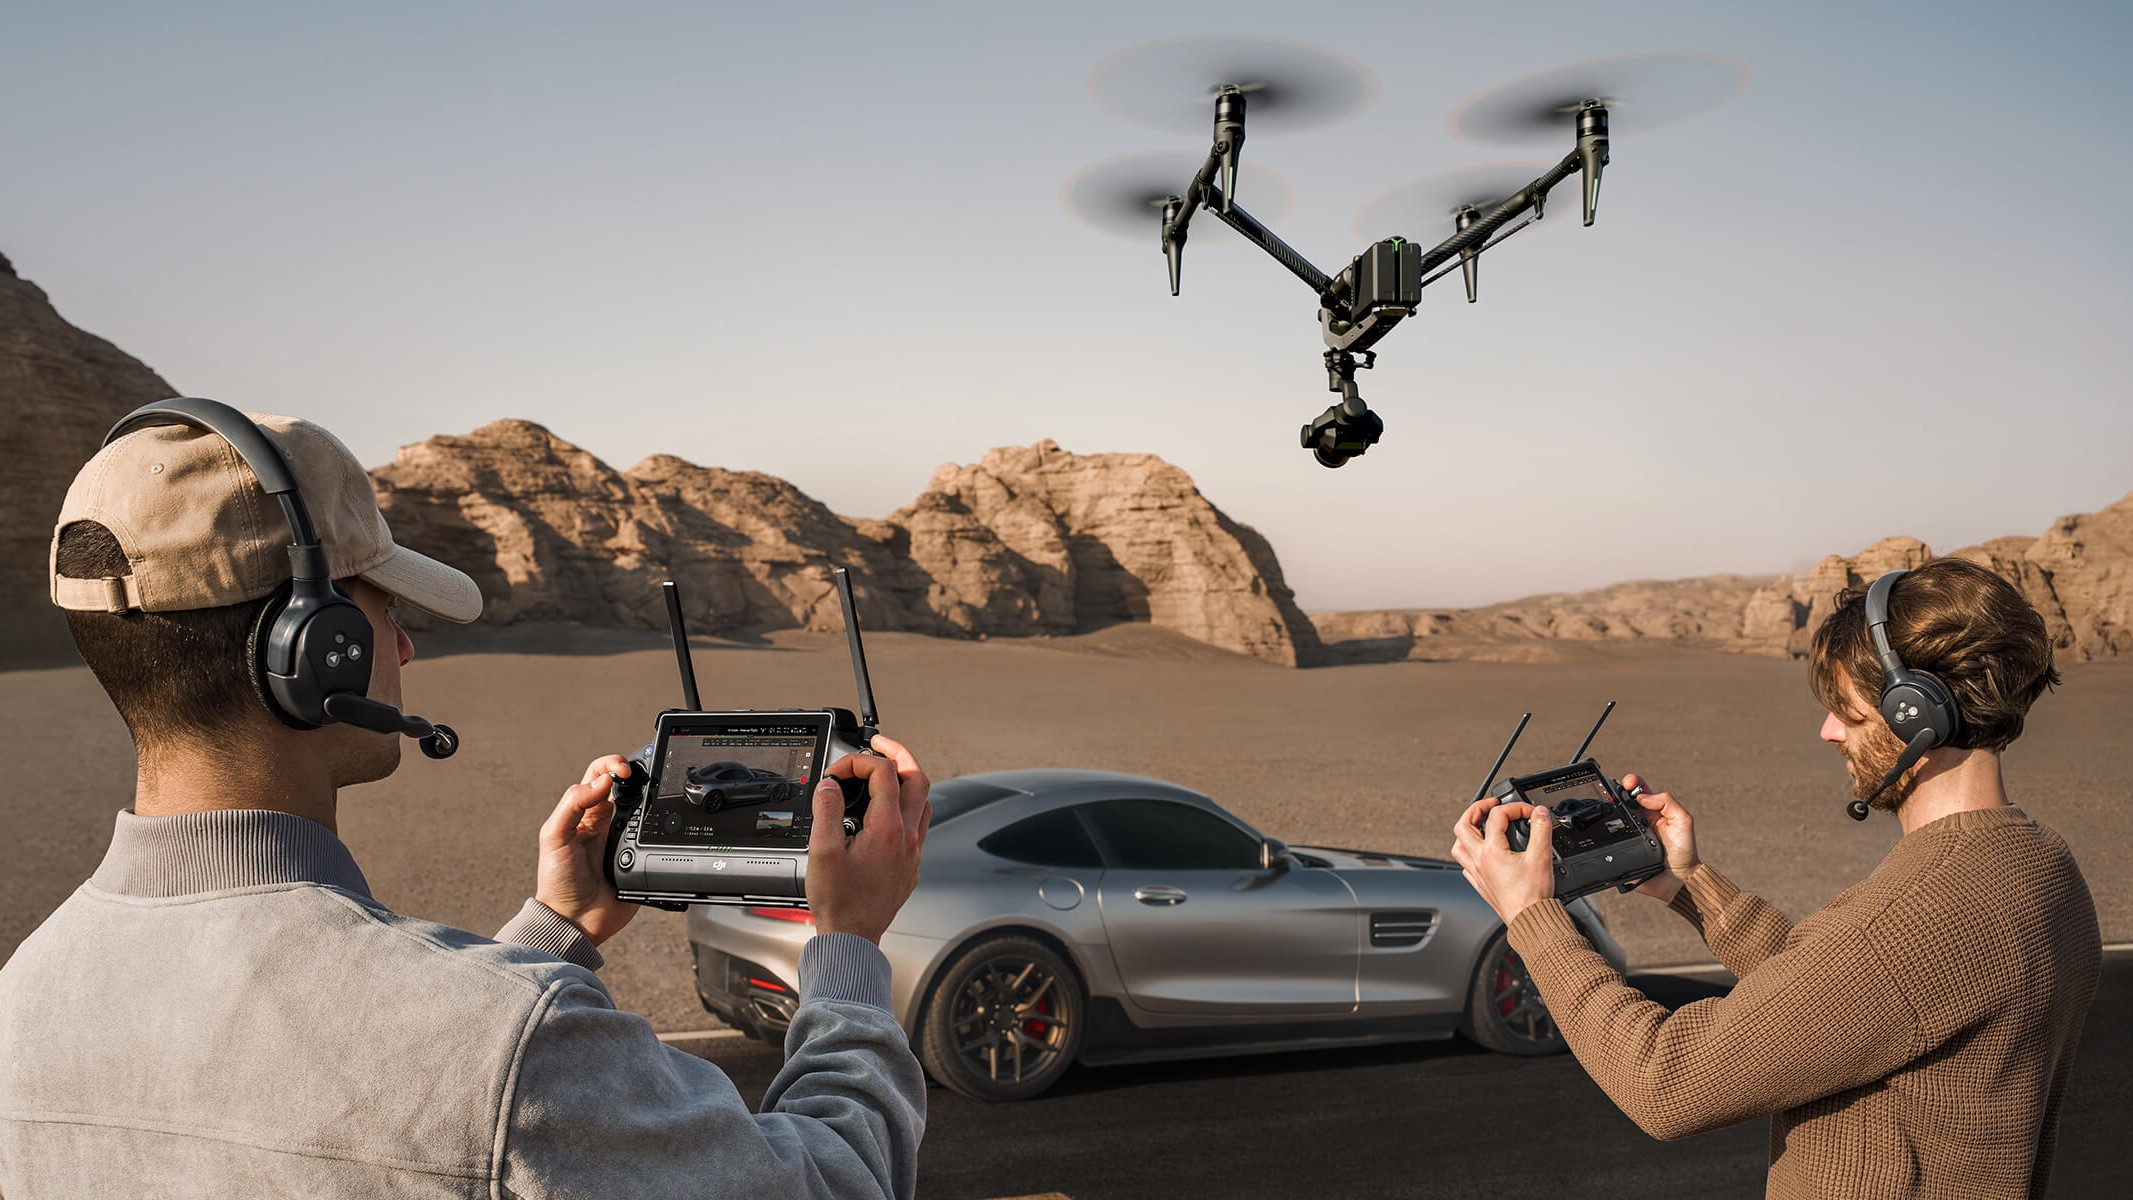
\includegraphics[width=\linewidth]{dji.jpg}
        \caption{航拍无人机拍摄电影\protect\footnotemark[1]}
        \label{dji}
    \end{minipage}
    \hfill % 在图片之间添加一些空间
    \begin{minipage}[b]{0.49\linewidth}
        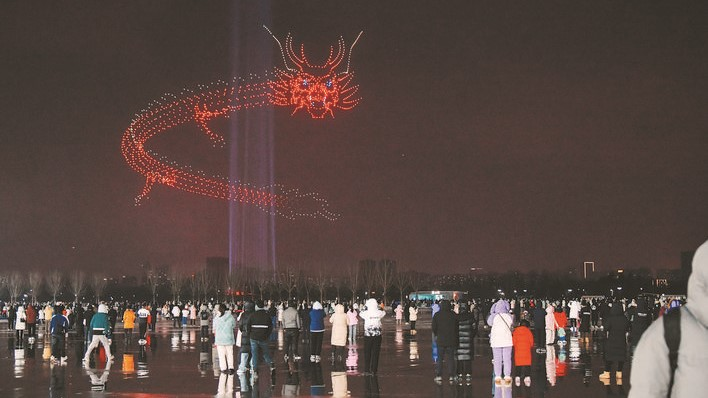
\includegraphics[width=\linewidth]{灯光秀.jpg}
        \caption{无人机集群灯光表演\protect\footnotemark[2]}
        \label{灯光秀}
    \end{minipage}

    %\vspace{1cm} % 在行之间添加一些垂直空间

    \begin{minipage}[b]{0.49\linewidth}
        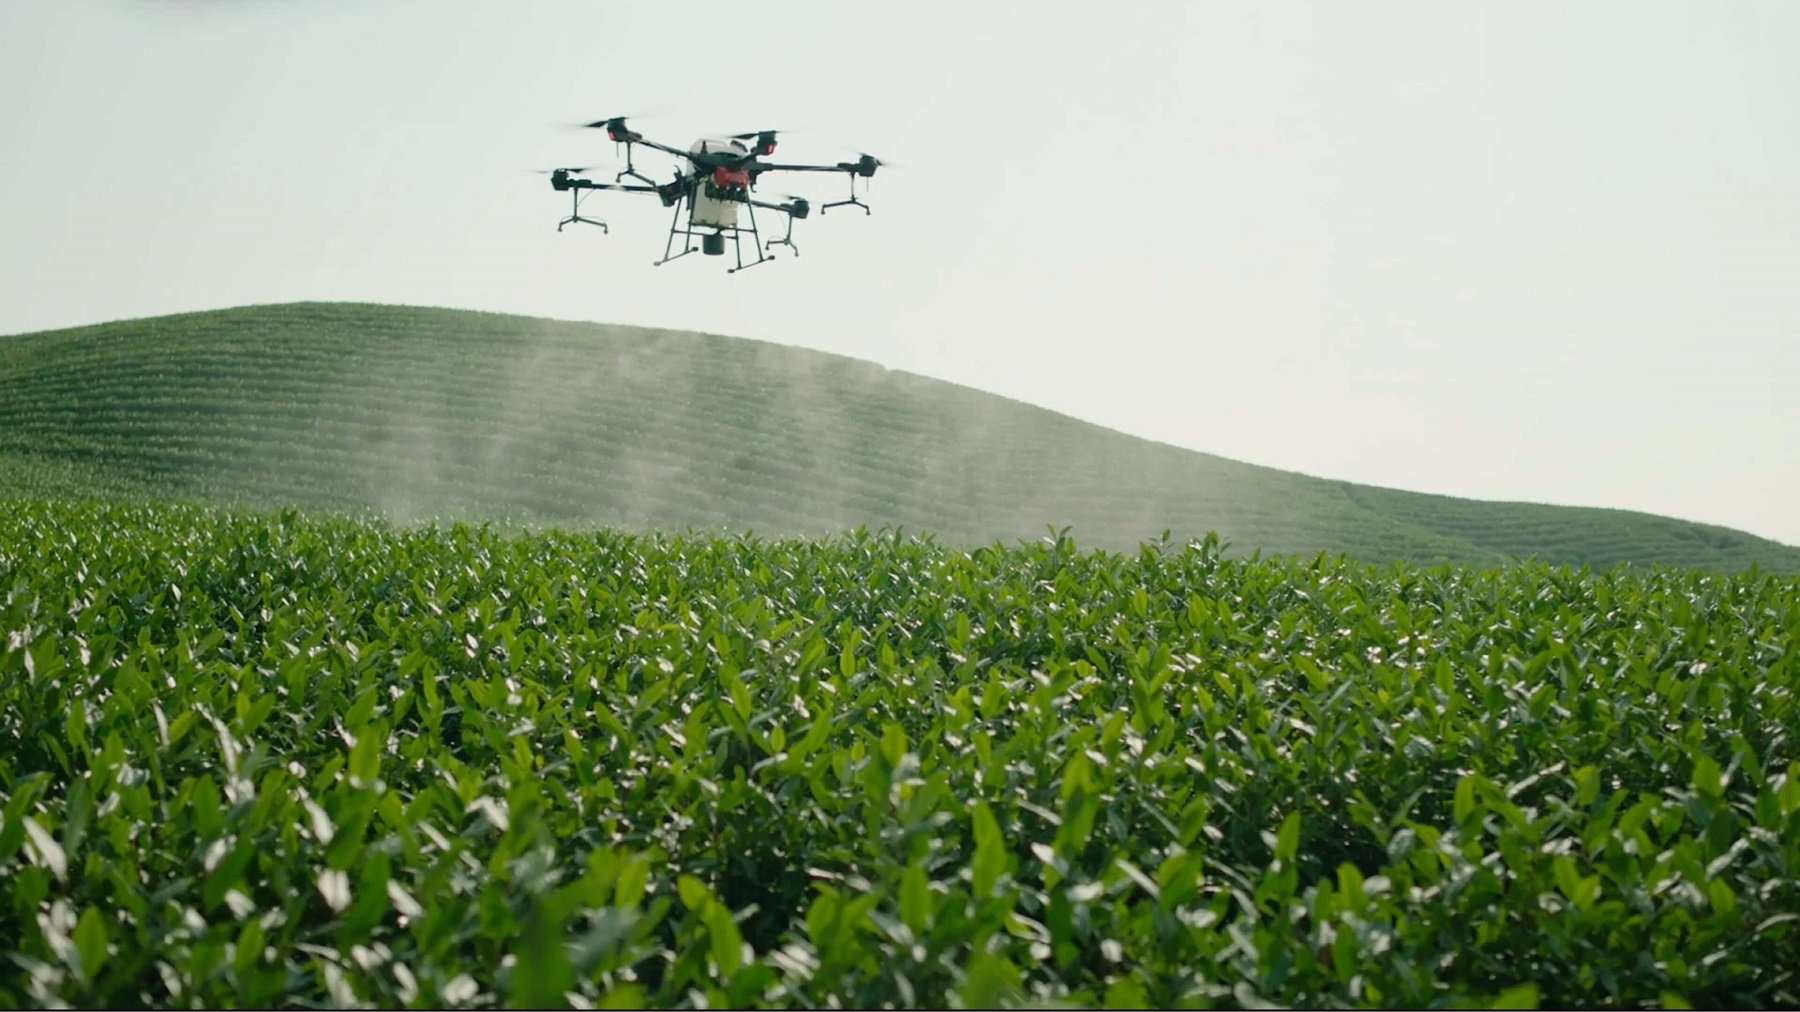
\includegraphics[width=\linewidth]{植保.jpg}
        \caption{植保无人机田间作业\protect\footnotemark[3]}
        \label{植保}
    \end{minipage}
    \hfill
    \begin{minipage}[b]{0.49\linewidth}
        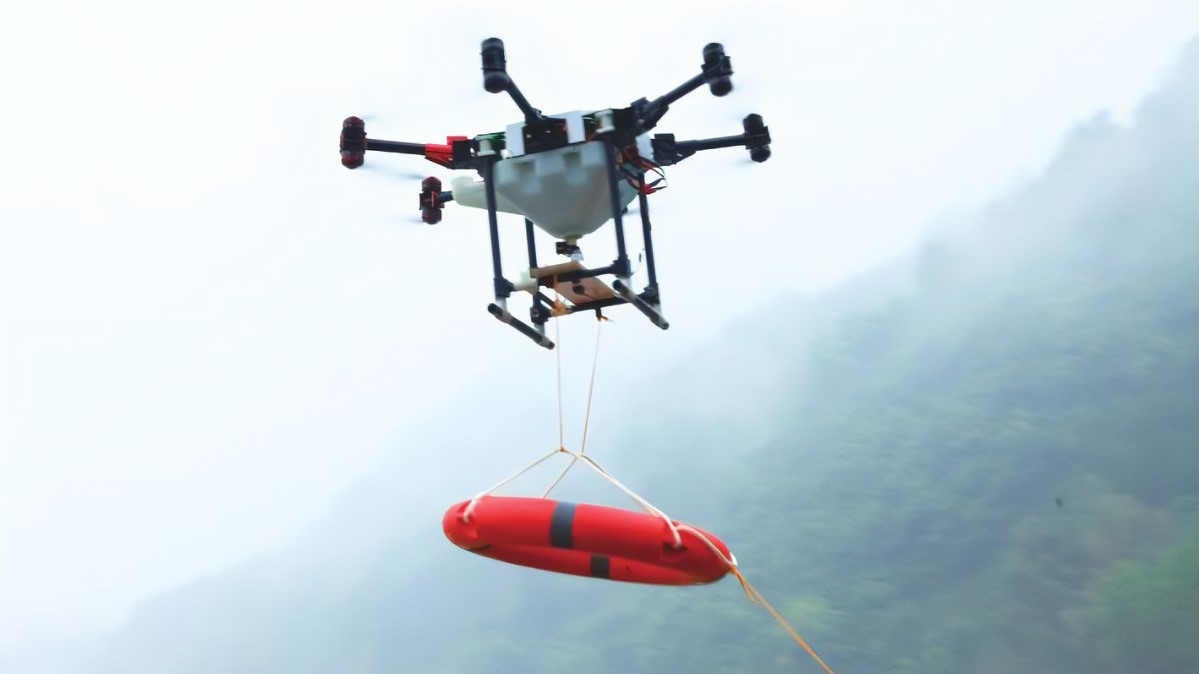
\includegraphics[width=\linewidth]{搜救.jpg}
        \caption{救援无人机水面营救\protect\footnotemark[4]}
        \label{救援}
    \end{minipage}
\end{figure}
\footnotetext[1]{图片来源:\url{https://www.dji.com/cn/inspire-3?site=brandsite&from=landing_page}}
\footnotetext[2]{图片来源:\url{https://www.scnjnews.com/content/2023-06/25/content_6509732.html}}
\footnotetext[3]{图片来源:\url{https://news.mydrivers.com/1/655/655677.htm}}
\footnotetext[4]{图片来源:\url{https://uav.huanqiu.com/article/9CaKrnK3V5e}}
尽管四旋翼无人机在许多领域都已经有了落地应用,但它们的飞行控制仍然有进步完善的空间。系统的高度非线性、大角度机动时的脆弱稳定性以及传感器对环境噪声的敏感性等仍然是无人机飞行控制要面临的技术难题。这些技术难题的存在,限制了无人机在更多高风险或复杂环境中的应用。因此,深入研究和优化四旋翼无人机的飞行控制技术,不仅能够推动无人机技术的进一步商业化,还有助于拓宽其在社会服务和经济活动中的应用范围,如更复杂的城市空中交通管理和多无人机协同作业等新兴领域。

综上所述,四旋翼无人机的研究不仅具有重要的技术意义,更在社会经济和安全等多个层面发挥着越来越重要的作用。因此,本研究旨在通过对四旋翼无人机飞行控制的深入分析和改进,解决现有的技术难题,为其更广泛的应用奠定坚实的基础。
\section{四旋翼飞行控制的研究现状}
四旋翼无人机出于上述的种种优势和应用场景,近年来得到了广泛研究\cite{survey}。四旋翼具有高度机动性的优势,同时也有欠驱动、载荷算力有限和高控制频率的限制。这使得四旋翼成为验证先进控制理论的理想测试平台\cite{La2018}。
   

随着近年来计算机处理能力的增强以及传感器的发展,关于无人机控制的研究快速发展。
2004年,Bouabdallah将角速度近似等于欧拉角的导数,得到简化后的四旋翼动力学方程,在此基础上他分步解决姿态跟踪和高度跟踪的问题。他使用了简单的闭环反馈作为控制器进行仿真和实机实验,证实了其控制姿态角的能力\cite{boua2007}。但这一阶段的工作还比较粗糙,在姿态角较大时将角速度近似等于欧拉角会带来很大的偏差。其控制器几乎只是依赖调参,抗扰动能力较差,并且也只做到了悬停的高度控制。于是在2005年,Bouabdallah进一步提出了反步法和滑膜控制两种非线性的方法\cite{boua2005},做到了四旋翼的位置控制并增强了抗扰动能力。虽然还是根据近似后的动力学模型,但反步法能够在较高扰动的情况下做到对方向角的控制。而滑膜控制由于开关特性引入了高频低振幅的振动,使得传感器漂移,导致控制效果一般。2007年在此基础上改进的积分反步法\cite{bouabdallah2007full},也就是在将角速度期望设为角度误差的PID,达成了更好的角度控制。但受限于电机的响应速度,抖动仍然存在。积分反步法也应用在了位置控制的环节,做到了自动起降、悬停和避障。这一系列的工作在当年是开创性的,但由于传感器精度和频率、执行器性能的限制,其表现在今天看来还是较为不足。


以上的工作对期望位姿的解算实质上是欠缺物理意义的,而T. Lee于2010年提出了针对四旋翼复杂机动的非线性控制\cite{Lee2010},在没有对动力学近似的情况下,对这个问题做了物理上合理的解答。由于四旋翼的合推力总是垂直于机身平面,所以将位置环通过前馈和反馈控制算出的期望推力方向作为期望的z轴指向,再由用户输入的期望机头朝向投影得到期望的x轴朝向,由此构建起了完整的期望姿态。接下来就要设计姿态的控制方法,T. Lee根据罗德里格斯公式,由旋转矩阵的迹得到等效绕轴旋转的角度,并将其作为误差。随后还是从李雅普诺夫稳定性出发设计姿态控制率,在一系列极为巧妙的数学推导后得到了指数收敛的控制器。该控制方法能够跟踪输入的三维的位置和一维的机头朝向,在几乎全局拥有指数收敛性,由仿真证实了其良好的效果。

同年,后来风靡全球的开源飞控PX4发布\cite{brescianini2013nonlinear},它将四旋翼的控制分为位置、速度、姿态、角速度四个环,每个环都只采用了简单的PID控制,便于普通用户调试且能很好地适配不同参数的航模。在最重要的姿态环,它简单地用四元数表示下的旋转作差得到期望的角速度。由于传感器技术的发展,IMU和陀螺仪的频率大幅增加,使得高频率的内环控制成为可能。

针对无人机模型参数不确定和存在测量噪声的情况,A. C. Satici提出的鲁棒最优控制器在$L_1$最优意义上使误差幅度呈指数下降,最小化系统相对于扰动的$L_\infty$增益\cite{satici2013robust}。
由于不同风况对无人机飞行的影响难以建模,所以Michael O'Connell提出了通过深度学习结合预训练的Neural-Fly\cite{o2022neural},来实现快速在线适应。Neural-Fly 实现了精确的飞行控制,跟踪误差比最先进的非线性控制器和自适应控制器还要小得多。除了强大的经验性能之外,Neural-Fly 的指数稳定性还带来了鲁棒性保证。

\section{高阶全驱系统理论}
高阶全驱系统(High-order Fully Actuated, HOFA)理论是段广仁院士提出的,有别于状态空间方法的新架构\cite{duan1}\cite{duan2}\cite{duan3}\cite{duan4}\cite{duan5},并且在一系列的论文中系统阐述了高阶全驱系统的控制设计方法、能控性能观性判据等问题\cite{段1}\cite{段2}。高阶全驱系统理论为控制系统,尤其是处理非线性动态系统提供了新的视角。这一理论将卡尔曼提出的传统的一阶系统方法扩展到高阶情况,其中系统由二阶或更高阶的微分方程描述。大多数由基本物理定律建模的物理系统,比如牛顿第二定律、刚体动力学欧拉方程和基尔霍夫定律,自然表现为二阶系统。因此,HOFA系统理论提供了一种更自然和直接的方法来理解和控制这些系统,而不用将原本的高阶方程升维降阶到一阶的状态空间范畴里再设计控制算法。高阶全驱系统理论提出了满足一定条件的非线性系统控制的基本流程,第一步将非线性系统转化为伪严格反馈系统,第二步建立系统的HOFA模型。一旦导出 HOFA 模型,就可以立即设计控制器,使闭环系统成为具有所需特征结构的恒定线性系统。还提供了闭环系统中存在的所有设计自由度,可以进一步利用这些自由度来实现额外的系统性能。

高阶全驱系统的理论方法在控制方面相较于状态空间表示拥有以下优势:1)一旦导出系统的单个HOFA模型或一组HOFA模型,就可以立即写出非线性系统的控制器。2)总能得到恒定的线性闭环系统,从而可以应用线性系统的分析和设计方法。3)可以指定所需的闭环特征结构,并提供所有设计自由度,可以进一步利用这些自由度来实现额外的系统设计要求。4)该方法解决了许多 Lyapunov 方法无法解决的非线性控制问题,因为 Lyapunov 方法严重依赖于系统中非线性函数的复杂度,而 HOFA 系统方法仅利用全驱特性,而不管系统中非线性函数的复杂度。

HOFA系统的特点是它们能够通过外部输入直接控制每个状态变量,这一特性基于全驱动属性。这个属性允许消除复杂的非线性动力学,简化控制设计并提高系统性能。高阶全驱系统理论的一个核心概念是全驱动概念,这一概念从根本上改变了控制设计的方法。与最适合状态响应分析的状态空间表示不同,HOFA模型在控制应用中表现出色,为控制器设计提供了一条直接的路径。HOFA方法在将系统表示为HOFA模型后,即可立即设计控制器。即使对于具有复杂非线性的系统,该模型也有效地线性化了控制过程。四旋翼的姿态环路就是一个全驱系统,可以应用高阶全驱系统理论,将原本的非线性系统转化为线性系统,随后可以方便地应用各种线性系统方法进行控制。

HOFA系统理论在机器人技术、航空航天和精密制造等多个领域有着广泛的应用。通过提供更直观和有效的控制设计方法,HOFA系统有潜力彻底改变我们分析、设计和实现控制系统的方式,以应对高阶和非线性动态。高阶全驱系统理论的发展标志着控制系统理论的重大进步。它不仅丰富了我们对复杂系统的理解,还提供了应对非线性和高阶动态挑战的实用工具。HOFA方法为控制系统设计提供了增强的能力,为各种工程领域的研究和应用开辟了新的途径。
\section{本文研究动机}
近年来,已经有许多控制方法被用于四旋翼无人机的飞行控制,其中既有各类非线性方法,包括$H_\infty$控制\cite{H}、MPC控制\cite{MPC}、滑模控制\cite{sliding}等,也有将四旋翼模型简化后的线性方法\cite{boua2007}。但非线性的方法失于复杂,不如线性系统有许多成熟可用的理论,而简化后的四旋翼的模型会丢失关键特性,使控制效果下降,尤其是在姿态角较大时。

因此,若能找到一种方法,无损地将四旋翼飞行器的原始非线性模型转换为线性系统,则可在充分发挥其优势的同时,避免其弊端。高阶全驱动系统理论恰好能够完美实现这一点。在四旋翼的姿态环控制中,控制器接收三自由度的期望姿态作为输入,输出三维的扭矩,完全符合全驱动系统的要求。通过使用姿态与角速度的组合来补偿系统的原有非线性,可以实现姿态控制环的线性化,从而便于采用线性控制方法来设计控制律。从理论上看,补偿后的姿态控制环将完全等同于一个线性环节,具备快速的动态响应和出色的稳态性能。一旦姿态控制环实现快速收敛,位置控制环的设计也将变得无障碍。
\section{本文研究内容和章节安排}
基于高阶全驱系统理论,本文对四旋翼的飞行控制展开了研究,在理论上设计了基于高阶全驱系统理论的最优控制器,通过Matlab仿真验证了控制器的优越性,随后展开了基于PX4和ROS的软件在环仿真,进一步进行了硬件在环仿真,搭建了室内基于动捕的无人机实验平台。本文提出的控制方法在接近理想的仿真环境中拥有相对的优越性,但在真实的实验场景下,由于时间的限制,尚有很多工程问题没有解决,还无法得到令人满意的效果。

第一章:介绍了四旋翼无人机的应用背景和研究意义,以及当前四旋翼无人机飞行控制的研究现状,介绍高阶全驱系统理论基础知识。阐述了本文的研究动机。对于四旋翼飞行控制的发展过程和研究现状进行了有针对性的文献调研和分析。

第二章:推导四旋翼的动力学模型,设计基于高阶全驱系统理论的四旋翼最优控制用于四旋翼的姿态环路。介绍Matlab下的数值仿真实验设计,与经典的SO(3)控制和PID控制对比,分析其收敛速度和跟踪精度,验证了理论设计的控制策略在模拟环境中的有效性。

第三章:讨论了基于ROS的半实物仿真设置,包括软件配置、算法实现和硬件集成,展示了实验结果,进一步证实了所提控制策略的实际应用潜力。

第四章:介绍了实机飞行平台的搭建和进行PX4原生固件轨迹跟踪实验的详细过程,通过分析实机飞行数据为本方法进一步的实机运行提供了参考。

第五章:总结本文工作,分析本研究工作的优点与不足,并对未来的研究方向提出展望。